\begin{quote}
Although a grounding in learning theory helps inform peer learning
projects, Peeragogy, at its core, comes to life in applied practice.
Even before convening a group for your peer learning project, you will
want to take a look over the patterns we have collected here. You will
likely return here many times as your project develops.

\end{quote}
\subsection{What is a pattern?}

A pattern is anything that has a repeated effect. In the context of
peeragogy, the practice is to repeat processes and interactions that
advance the learning mission. Frequent occurrences that are not
desirable are called anti-patterns!

\begin{quote}
\textbf{Christopher Alexander}: ``Each pattern describes a problems
which occurs over and over again in our environment, and then describes
the core of the solution to that problem, in a way that you can use this
solution a million times over, without ever doing it the same way
twice.'' {[}1{]}

\end{quote}
Patterns provide a framework that can be applied to similar issues but
may be metaphorically solved in different ways, sometimes in real world
or face to face events and other times in digital space. Outside of
Alexander's own work in architecture, one the first groups to adopt a
design pattern way of thinking about things were computer programmers.
Writing in the foreward to Richard P. Gabriel's \emph{Patterns of
Software}, Alexander emphasizes that the key question to ask about any
design approach is: does it help us build better?

\begin{quote}
\textbf{Christopher Alexander}: ``What is the Chartres of programming?
What task is at a high enough level to inspire people writing programs,
to reach for the stars?'' {[}2{]}

\end{quote}
We think that Peeragogy stands a good chance of being a ``killer app''
for pattern-based design. Learning bridges physical and virtual worlds
all the time. And, in fact, a \emph{Network of Learning} was the 18th
pattern that Christopher Alexander introduced in his book, \emph{A
Pattern Language}.

\begin{quote}
\textbf{Christopher Alexander}: ``Work in piecemeal ways to decentralize
the process of learning and enrich it through contact with many places
and people all over the city: workshops, teachers at home or walking
through the city, professionals willing to take on the young as helpers,
older children teaching younger children, museums, youth groups
travelling, scholarly seminars, industrial workshops, old people, and so
on.'' {[}1{]}

\end{quote}
Peeragogy can help to extend and enrich this network, and, as we shall
see, patterns can be used by those involved to do ongoing ``emergent''
design, not only by building new structures, but by adapting and
improving our catalog of patterns as we go.

\subsection{Patterns of peeragogy}

Here is our index of the main patterns we've found so far (described in
more detail after the jump):

\begin{itemize}
\item
  \textbf{\href{http://peeragogy.org/patterns/wrapper/}{Wrapper}} - Front end
  appearance to participants. Consolidate and summarize.
\item
  \textbf{\href{http://peeragogy.org/patterns/discerning-a-pattern/}{Discerning
  a pattern}} - Found a pattern? Give it a title and record an example.
  (Woah, meta!)
\item
  \textbf{\href{http://peeragogy.org/patterns/polling-for-ideas/}{Polling for
  ideas}} - Invite brainstorming, collecting ideas, questions, and
  solutions.
\item
  \textbf{\href{http://peeragogy.org/patterns/creating-a-guide/}{Creating a
  guide}} - Overviews expose the lay of the land. Collecting content and
  stories.
\item
  \textbf{\href{http://peeragogy.org/patterns/newcomer/}{Newcomer}} - Create a
  guide for ``beginner's mind'' and help avoid need to introduce new
  members each ``meeting.''
\item
  \textbf{\href{http://peeragogy.org/patterns/roadmap/}{Roadmap}} - Plans for
  future work, direction towards a goal, dynamic
\item
  \textbf{\href{http://peeragogy.org/patterns/roles/}{Roles}} - Specialize and
  mix it up. Play to participants strengths and skills.
\item
  \textbf{\href{http://peeragogy.org/focusing-on-a-specific-project/}{Project
  focus}} - Lightbulb moment: Most specific projects involve learning!
\item
  \textbf{\href{http://peeragogy.org/patterns/carrying-capacity/}{Carrying
  capacity}} - Know your limits, find ways to get other people involved.
\item
  \textbf{\href{http://peeragogy.org/patterns/heartbeat/}{Heartbeat}} - The
  ``heartbeat'' of the group keeps energy flowing.
\item
  \textbf{\href{http://peeragogy.org/patterns/moderation/}{Moderation}} - When
  leaders step back, dynamics can improve; moderator serves as champion
  and editor.
\item
  \textbf{\href{http://peeragogy.org/patterns/praxis-vs-poeisis/}{Use or make?}}
  - Repurposing, tinkering, or creating from scratch?
%% \item
%%   \textbf{\href{http://peeragogy.org/reiterate/}{Reiterate} - Periodically
%%   review and revise actions as needed
\end{itemize}
We'll introduce three additional patterns in the chapter on
\href{http://peeragogy.org/to-peeragogy/researching-peeragogy/}{researching
peeragogy}.

\subsection{Anti-patterns for Peeragogy}

And some ``anti-patterns'' (things to avoid if possible):

\begin{itemize}
\item
  \textbf{\href{http://peeragogy.org/antipatterns/isolation/}{Isolation}} - A
  tale of silos, holes, and not-invented-here.
\item
  \textbf{\href{http://peeragogy.org/antipatterns/magical-thinking/}{Magical
  thinking}} - ``One meeting will (not) change everything!''
\item
  \textbf{\href{http://peeragogy.org/antipatterns/co-learning-messy-with-lurkers/}{Messy
  with Lurkers}} - What happens when joining is low-cost and completion
  is low-benefit.
\item
  \textbf{\href{http://peeragogy.org/antipatterns/misunderstanding-power/}{Misunderstanding
  Power}} - The workload is almost never evenly distributed.
\item
  \textbf{\href{http://peeragogy.org/antipatterns/navel-gazing/}{Navel Gazing}} -
  ``I have this really great idea\ldots{}''
\item
  \textbf{\href{http://peeragogy.org/antipatterns/stasis/}{Stasis}} - What is the
  driver behind open source, commons-oriented collaborative projects?
  (Because, let's face it, it doesn't always work.)
\item
  \textbf{\href{http://peeragogy.org/antipatterns/stuck-at-the-level-of-weak-ties/}{Stuck
  at the level of weak ties}} - Can we deepen the connection?
\end{itemize}
\subsection{What is a use case?}

A use case describes someone (or something) who uses a given system or
tool to achieve a goal. A use case can include a title, a summary of the
problem, an actor, and a success scenario. Additional features can be
added, such as alternate interactions or choices that lead to a
variation on the result.

The use case considers a given persona (a characteristic role) in a
given situation and shows how they works on a project/problem and how
their process of work is resolved into a solution or solutions. Some
activities do not have a single solution -- these are often referred to
as ``Wicked Problems.'' With detailed bookkeeping effort, recorded
processes can be standardized into use cases that can then be employed
directly or modified to fit the context of the activity at hand. In
short, they are a lot like design patterns, which they may contain in
hidden or explicit form. Use cases are presented in vignettes that
appear throughout the book (like the one at the end of this section).

\subsection{A peeragogy pattern language}

By looking at how patterns combine in real and hypothetical use cases,
you can start to identify a \emph{pattern language} that can be used in
your projects. We can get a simplified view of these connections with
the following diagram. It's important to clarify that everyone doesn't
do it the same way. Here, the \emph{Roadmap} is given a central
position, but some peer learning projects will forego making a specific,
detailed plan; their plan is just to see what develops. You can see here
how peeragogy patterns often break down further into individual
micro-steps: we'll say more about that shortly.

\begin{figure}[htbp]
\centering
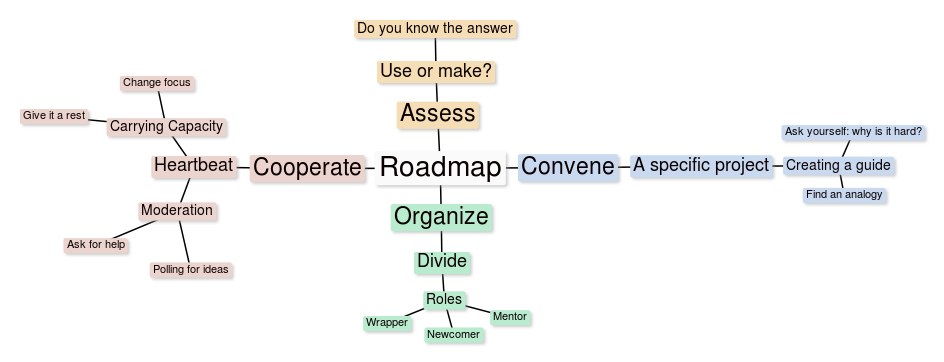
\includegraphics[width=\textwidth]{../pictures/pattern-language.jpg}
%\caption*{A map of some of the main features of our pattern language}
\end{figure}

The subsequent main sections of this book --
\href{http://peeragogy.org/convene/}{\emph{Convene}},
\href{http://peeragogy.org/organize/}{\emph{Organize}},
\href{http://peeragogy.org/facilitate/}{\emph{Cooperate}} and
\href{http://peeragogy.org/assessment/}{\emph{Assess}} -- represent big
clusters of patterns that are likely to come up time and again in
various projects. We can think of these as East, South, West, and North
in the diagram above. You are of course encouraged to invent your own
patterns and to connect them in new ways. Each project has a unique
design, and it's own unique way in which things play out in practice.
What we've put together here is a starter kit.

\begin{quote}
\textbf{Christopher Alexander}: These ideas---patterns---are hardly more
than glimpses of a much deeper level of structure, and is ultimately
within this deeper level of structure, that the origin of life occurs.
{[}2{]}
\end{quote}
\subsection{Patterns and Problem Solving}

Ten potentially useful things to do when you're solving a problem are
described by the computer scientist Marvin Minsky in a series of
\href{http://web.media.mit.edu/~minsky/OLPC-1.html}{m}\href{http://web.media.mit.edu/~minsky/OLPC-2.html}{e}\href{http://web.media.mit.edu/~minsky/OLPC-3.html}{m}\href{http://web.media.mit.edu/~minsky/OLPC-4.html}{o}\href{http://web.media.mit.edu/~minsky/OLPC-5.html}{s}
written for the One Laptop Per Child project. We can sum them up
visually with the following diagram:

\begin{figure}[htbp]
\centering
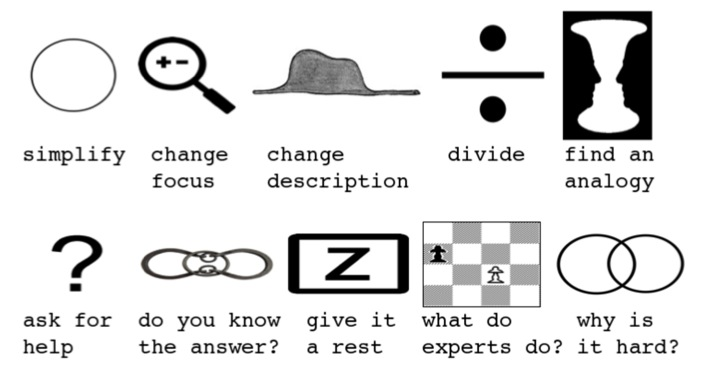
\includegraphics[width=\textwidth]{../pictures/heuristic-images.jpg}
\caption*{}
\end{figure}

We can also see some interesting connections between these intuitive
problem solving heuristics and peeragogy patterns listed above. This can
help illustrate further connections between the patterns, and some of
the ways that groups can apply them to solve real-world problem. To
elaborate briefly:

\begin{itemize}
\item
  Simplify things for \textbf{Newcomers}. We don't expect a newcomer to
  enter at full speed.
\item
  Use a \textbf{Roadmap} to guide us from one phase to another, while
  the project's central \textbf{Heartbeat} helps us attend to the
  central focus.
\item
  Announce changes through a \textbf{Wrapper} who describes the new
  status or direction of the project. For the Peeragogy project, that
  often meant summing up the high points that we saw over a given period
  of time.
\item
  We divide work up not only horizontally among different
  \textbf{Roles}, but also temporally by using the \textbf{Roadmap}.
  Someone who is moving ahead with the Roadmap is likely to be working
  at the leading edge.
\item
  When we find an analogy, we are basically \textbf{Creating a Guide}
  for thinking about something. This can be used as a form of
  ``exploration,'' as we look at how one form of engagement may or may
  not map onto other forms of engagement.
\item
  When we ask for help, we may avail ourselves of some
  \textbf{Moderation} service that will decide how to deal with our
  request. One simple way to ask for help is \textbf{Polling for Ideas}.
  Obviously once we start to get help, we're working in a regime of
  ``collaborative effort''.
\item
  If you know the answer, then you may be able to reuse it (which is the
  basic idea described in \textbf{Use or Make}.
\item
  It is important to give it a rest so as not to over-exhaust oneself,
  busting one's own \textbf{Carrying Capacity}, or, alternatively,
  overwhelming the group.
\item
  It seems that one of the things that experts are good at is
  \textbf{Discerning a Pattern}. This allows them to simplify their
  processing.
\item
  Finally, again, if we know why it is hard, then we may be able to
  \textbf{Create a Guide} that will help get around, or at least better
  cope with, the difficulty.
\end{itemize}

\subsubsection{References}

\begin{enumerate}
\item
  Alexander, Christopher, Ishikawa, Sara, and Silverstein, Murray,
  \emph{A Pattern Language: Towns, Buildings, and, Construction}, New
  York: Oxford University Press, 1977.
\item
  Gabriel, Richard P.
  \emph{\href{http://dreamsongs.net/Files/PatternsOfSoftware.pdf}{Patterns
  of Software}}, New York: Oxford University Press, 1996. (Includes a
  forward by Christopher Alexander.)
\end{enumerate}
